\subsection{Testing}
\subsubsection{Analisi Statica - CodeMR}

Questa sezione documenta l'analisi statica del codice eseguita con CodeMR per l'iterazione 2.

\begin{figure}[H]
    \centering
    \begin{minipage}{0.45\textwidth}
        \centering
        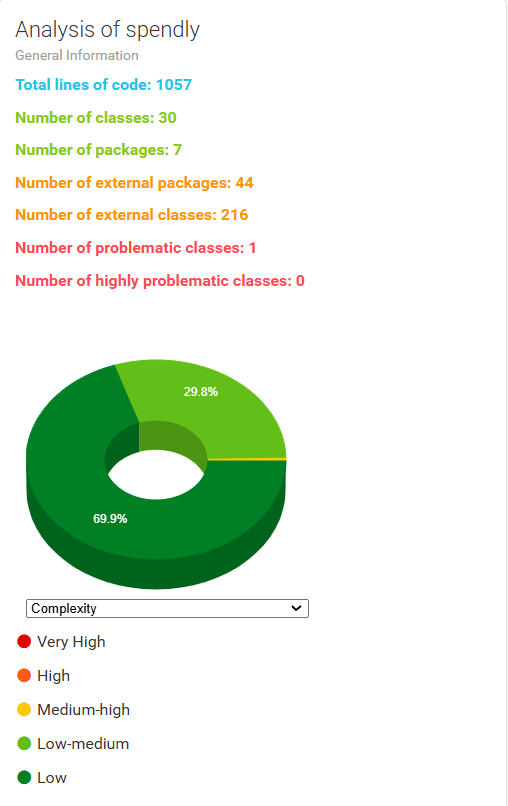
\includegraphics[width=\textwidth]{images/Complexity_iter2.png}
        \caption{Complexity}
        \label{fig:Complexity_iterazione2}
    \end{minipage}
    \hfill
    \begin{minipage}{0.45\textwidth}
        \centering
        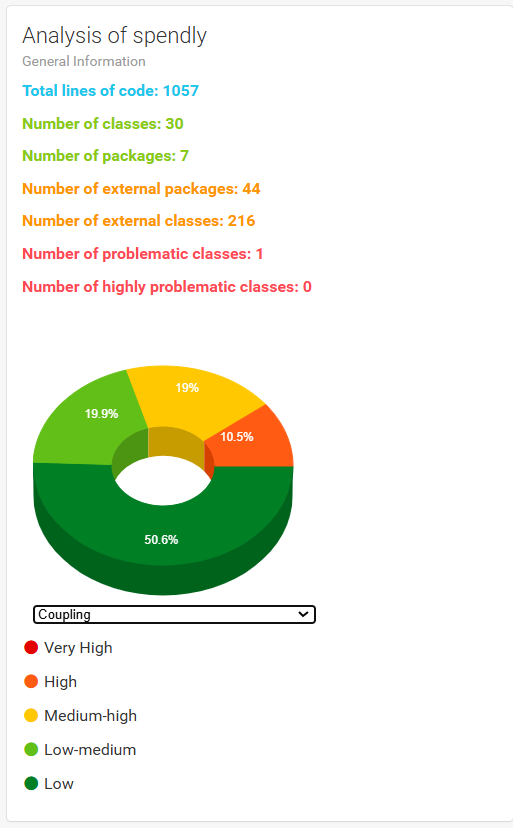
\includegraphics[width=\textwidth]{images/Coupling_iter2.png}
        \caption{Coupling}
        \label{fig:Coupling_iterazione2}
    \end{minipage}
\end{figure}

\begin{figure}[H]
    \centering
    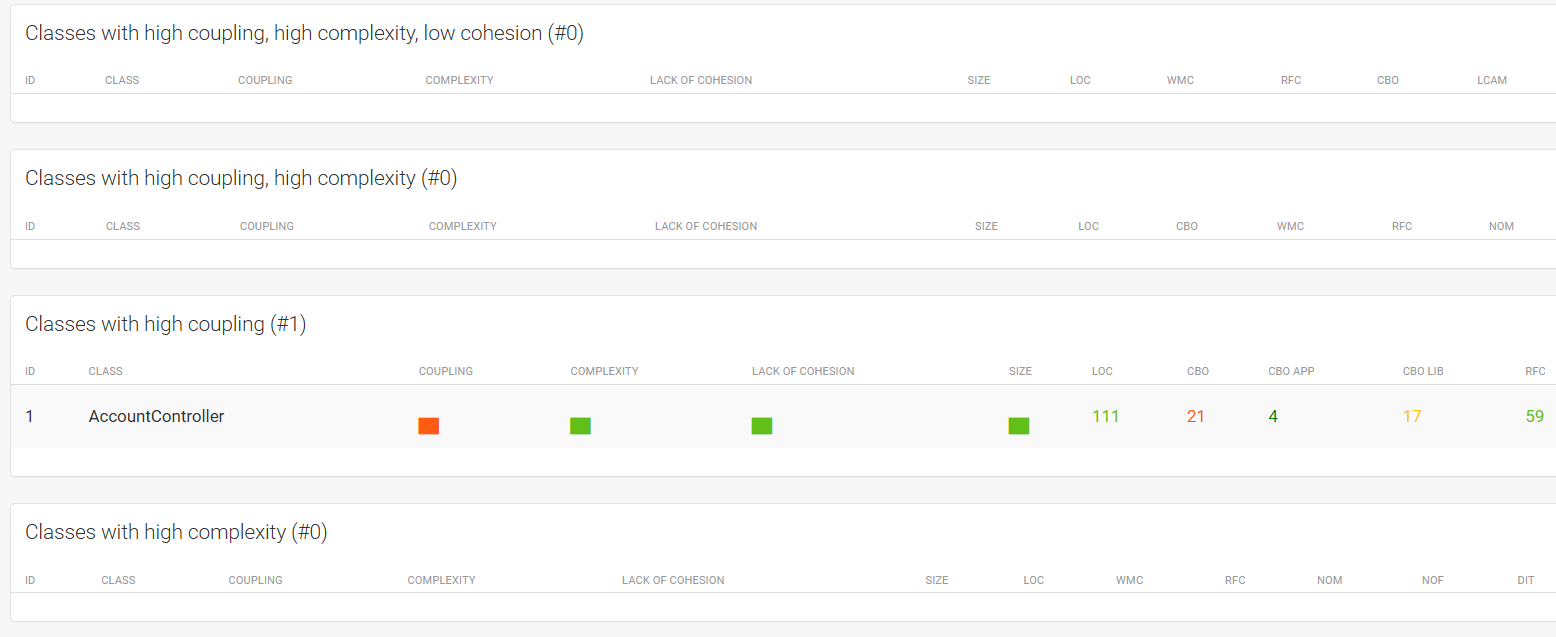
\includegraphics[width=1\textwidth]{images/Problem_iter2.png}
    \caption{Problemi classi}
    \label{fig:Problemi_iterazione2}
\end{figure}


\begin{figure}[H]
    \centering
    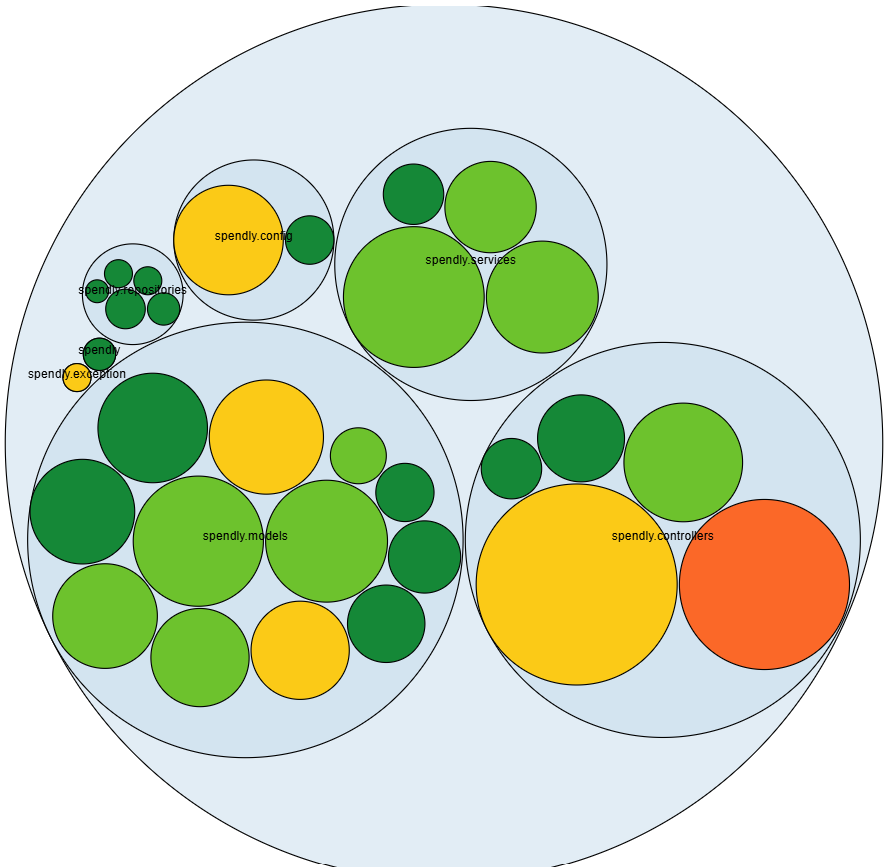
\includegraphics[width=0.8\textwidth]{images/Package_iter2.png}
    \caption{Struttura dei package}
    \label{fig:Package_iterazione2}
\end{figure}

\subsubsection{Analisi Dinamica - JUnit}

Questa sezione documenta i test d'unità implementati per l'iterazione 2. Sono stati aggiornati i test riguardanti i gruppi e sono stati implementati i test relativi ai costi.

\begin{figure}[H]
    \centering
    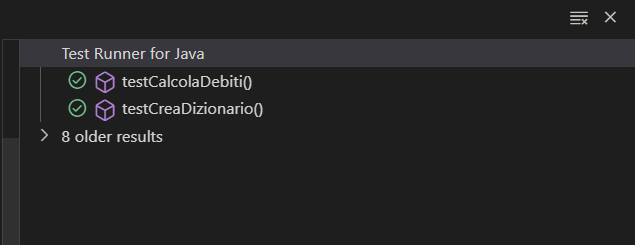
\includegraphics[width=0.9\textwidth]{images/CalcolaDebitiTest.png}
    \caption{Test per ottimizzare Debiti}
    \label{fig:CalcolaDebitiTest}
\end{figure}

\begin{figure}[H]
    \centering
    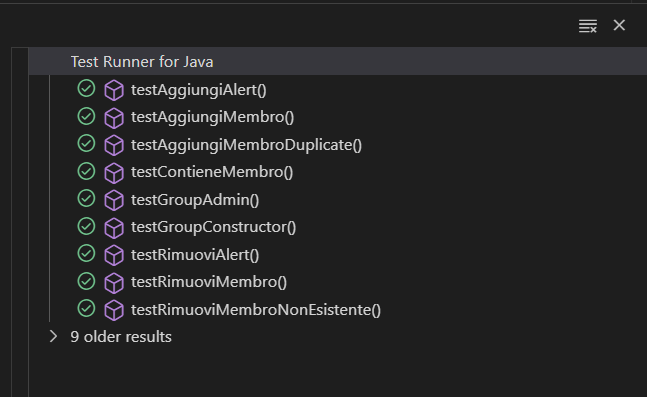
\includegraphics[width=0.9\textwidth]{images/GroupTest_iter2.png}
    \caption{Test aggiornati per la classe Group}
    \label{fig:GroupTest_iter2}
\end{figure}

\begin{figure}[H]
    \centering
    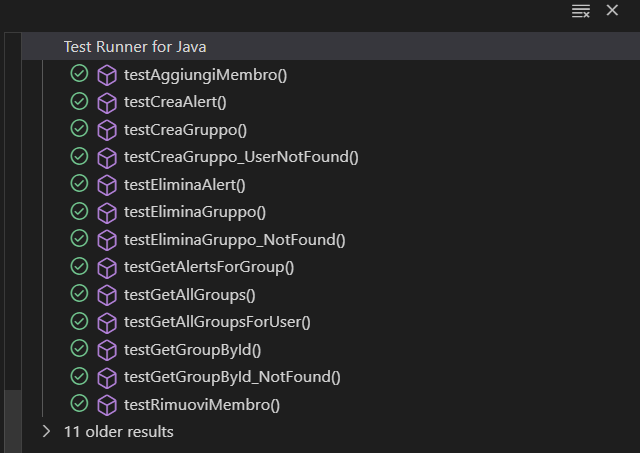
\includegraphics[width=0.9\textwidth]{images/GroupServiceTest_iter2.png}
    \caption{Test aggiornati per la classe GroupService}
    \label{fig:GroupServiceTest_iter2}
\end{figure}

\begin{figure}[H]
    \centering
    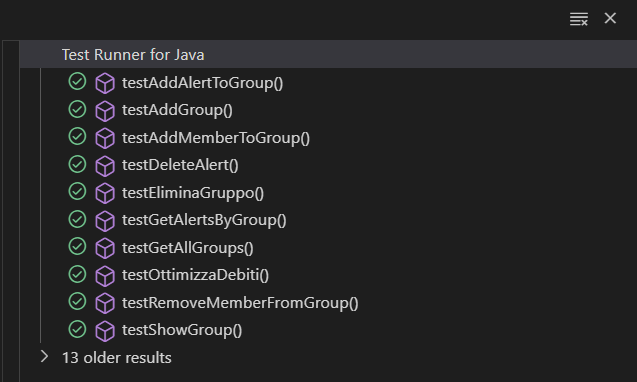
\includegraphics[width=0.9\textwidth]{images/GroupControllerTest_iter2.png}
    \caption{Test aggiornati per la classe GroupController}
    \label{fig:GroupControllerTest_iter2}
\end{figure}

\begin{figure}[H]
    \centering
    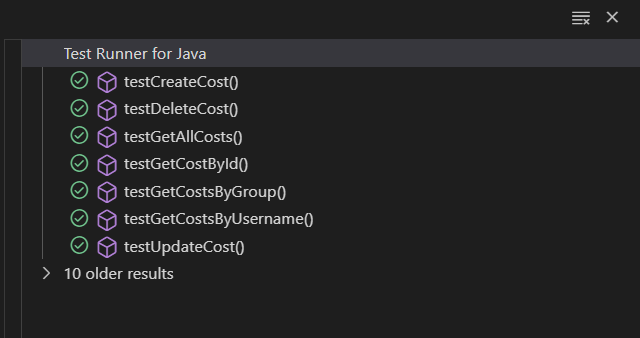
\includegraphics[width=0.9\textwidth]{images/CostServiceTest_iter2.png}
    \caption{Test per la classe CostService}
    \label{fig:CostServiceTest_iter2}
\end{figure}

\begin{figure}[H]
    \centering
    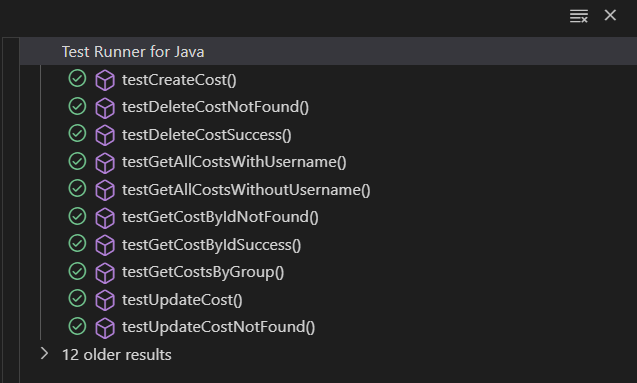
\includegraphics[width=0.9\textwidth]{images/CostControllerTest_iter2.png}
    \caption{Test per la classe CostController}
    \label{fig:CostControllerTest_iter2}
\end{figure}



\subsubsection{API Costi}

Questa sezione documenta le API relative alla gestione dei costi e degli alert  nel sistema Spendly, inclusi la creazione, l'eliminazione e la visualizzazione dei costi di utenti e gruppi. Ogni test verrà mostrato con un'immagine dei risultati.

\paragraph{Aggiunta di un Costo}  

\begin{itemize}
    \item \textbf{Endpoint:} \texttt{POST /api/costs?username=\{username\}}
    \item \textbf{Descrizione:} Permette all'utente autenticato di aggiungere un nuovo costo, eventualmente associandolo a un gruppo.
    \item \textbf{Parametri:}
    \begin{itemize}
        \item \texttt{importo} (double) - Importo della spesa.
        \item \texttt{tipologia} (string) - Tipo di spesa.
        \item \texttt{groupId} (integer, opzionale) - ID del gruppo a cui associare il costo.
    \end{itemize}
\end{itemize}
\newpage
\begin{figure}[h!]
    \centering
    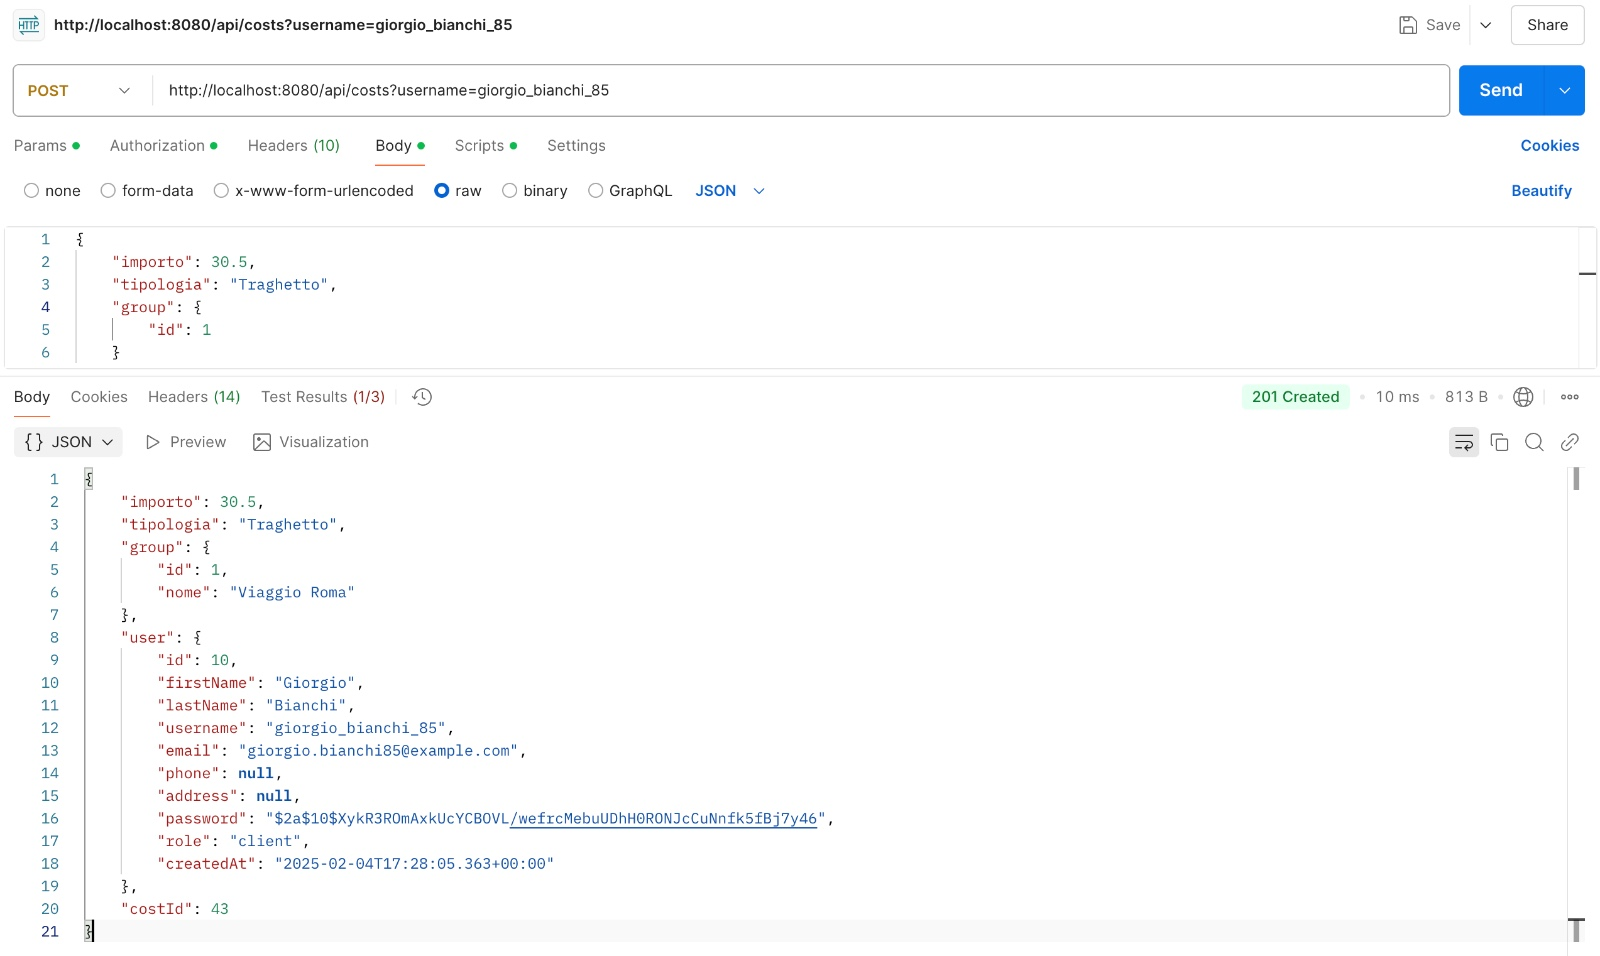
\includegraphics[width=0.9\textwidth]{images/createCost.jpeg}
    \caption{Risultato API Aggiunta Costo}
    \label{fig:api_add_cost}
\end{figure}

\paragraph{Eliminazione di un Costo}  

\begin{itemize}
    \item \textbf{Endpoint:} \texttt{DELETE /api/costs/\{costId\}}
    \item \textbf{Descrizione:} Permette all'utente autenticato di eliminare un costo precedentemente registrato.
    \item \textbf{Parametri:}
    \begin{itemize}
        \item \texttt{\{costId\}} (integer) - ID del costo da eliminare.
    \end{itemize}
\end{itemize}

\begin{figure}[h!]
    \centering
    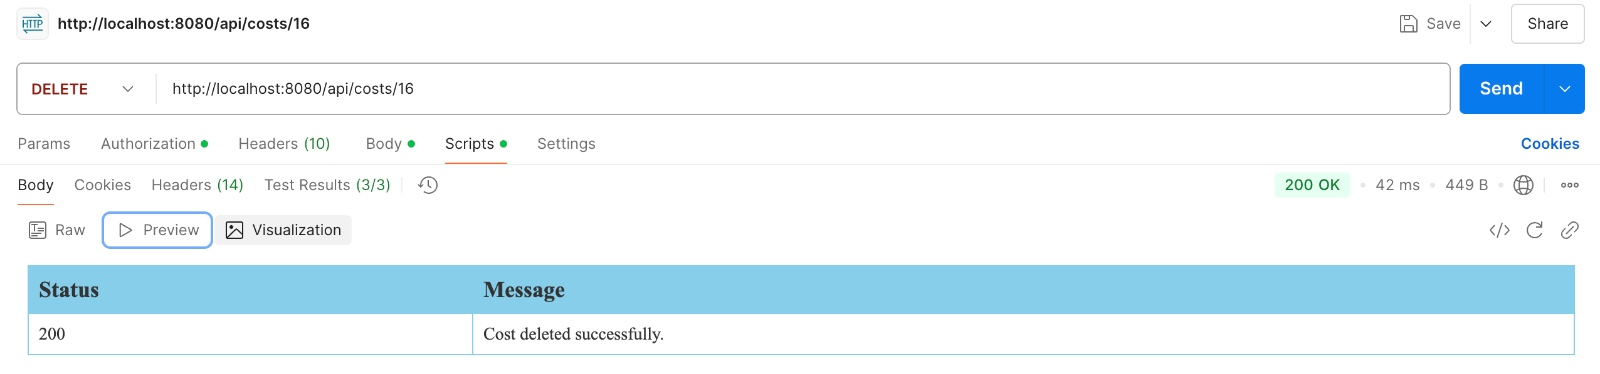
\includegraphics[width=0.9\textwidth]{images/deleteCost.jpeg}
    \caption{Risultato API Eliminazione Costo}
    \label{fig:api_delete_cost}
\end{figure}

\paragraph{Visualizzazione Costi Utente}  

\begin{itemize}
    \item \textbf{Endpoint:} \texttt{GET /api/costs?username=\{username\}}
    \item \textbf{Descrizione:} Restituisce la lista di tutti i costi registrati dall'utente autenticato.
\end{itemize}

\begin{figure}[h!]
    \centering
    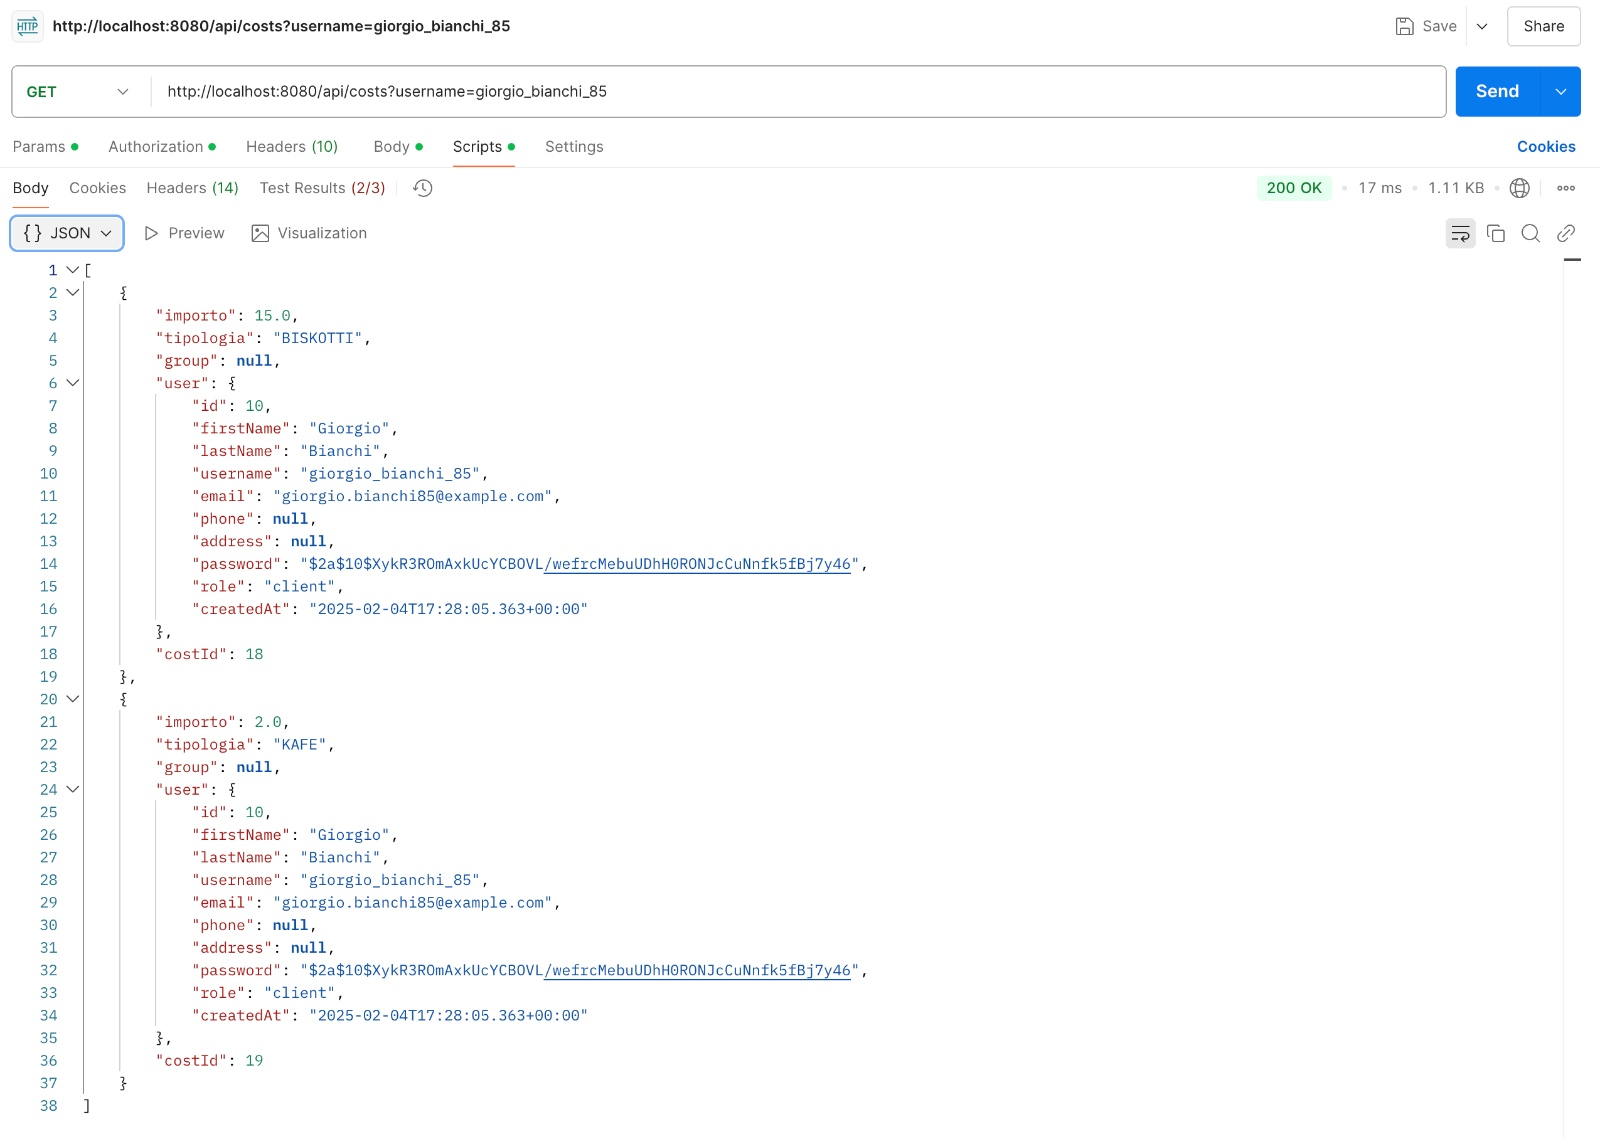
\includegraphics[width=0.9\textwidth]{images/getUserCosts.jpeg}
    \caption{Risultato API Visualizzazione Costi Utente}
    \label{fig:api_view_user_costs}
\end{figure}

\paragraph{Visualizzazione Costi di un Gruppo}  

\begin{itemize}
    \item \textbf{Endpoint:} \texttt{GET /api/costs/group/\{groupId\}}
    \item \textbf{Descrizione:} Restituisce la lista di tutti i costi registrati del gruppo.
\end{itemize}

\begin{figure}[H]
    \centering
    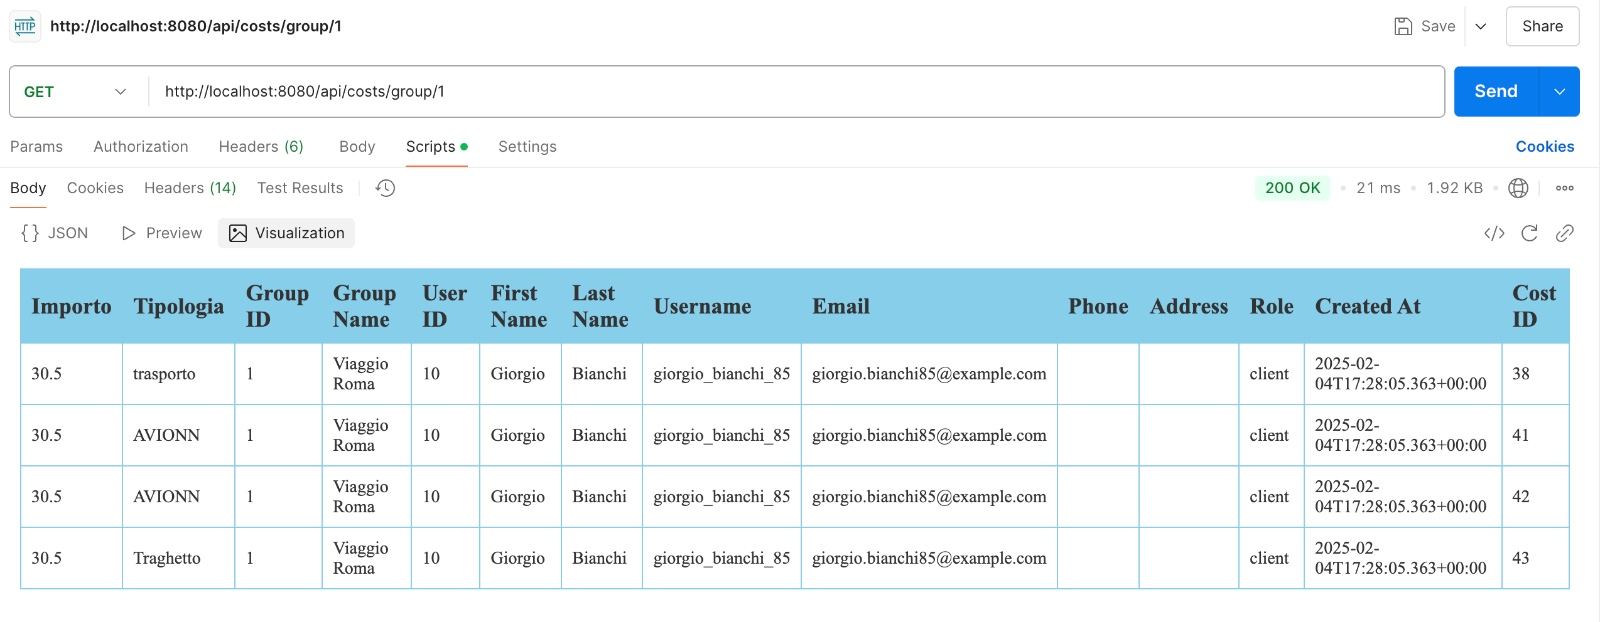
\includegraphics[width=0.9\textwidth]{images/getGroupCosts.jpeg}
    \caption{Risultato API Visualizzazione Costi Gruppo}
    \label{fig:api_view_group_costs}
\end{figure}


\paragraph{Creazione Alert} 

\begin{itemize}
    \item \textbf{Endpoint:} \texttt{POST /api/groups/\{groupId\}/alerts}
    \item \textbf{Descrizione:} Permette all'amministratore del gruppo di creare un Alert.
    \item \textbf{Parametri:}
    \begin{itemize}
        \item \texttt{adminUsername} (String) - Username admin del gruppo.
        \item \texttt{nome} (String) -Nome alert.
        \item \texttt{limite} (double) - Limite alert.
        \item \texttt{macroArea} (enum) - Area alert.
    \end{itemize}
\end{itemize}

\begin{figure}[H]
    \centering
    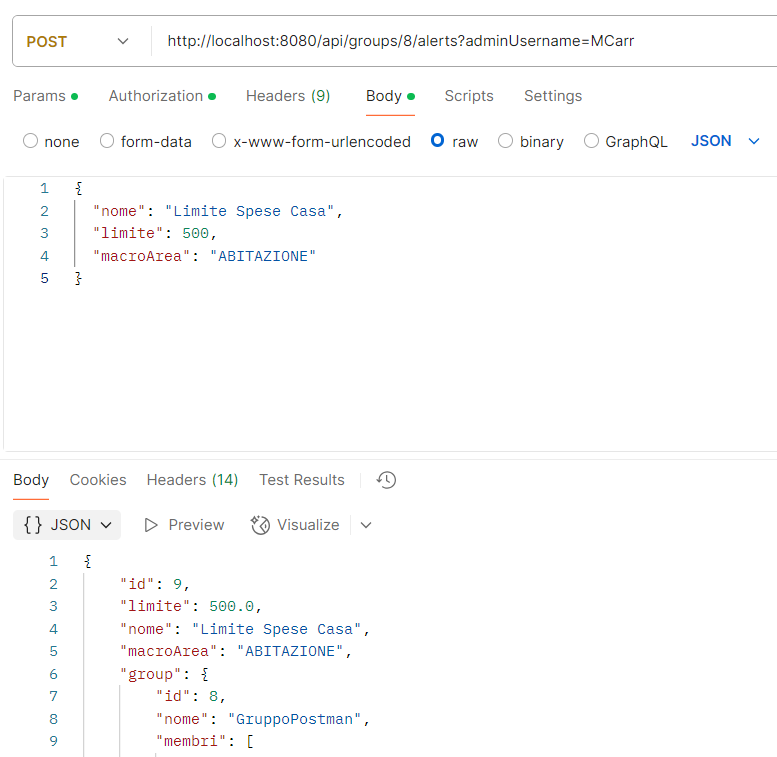
\includegraphics[width=0.9\textwidth]{images/createAlert.png}
    \caption{Risultato API Creazione Alert}
    \label{fig:api_createAlert}
\end{figure}

\paragraph{Eliminazione Alert}

\begin{itemize}
    \item \textbf{Endpoint:} \texttt{DELETE /api/groups/{groupId}/alerts/{alertId}}
    \item \textbf{Descrizione:} Permette all'amministratore del gruppo di eliminare un Alert.
    \item \textbf{Parametri:}
    \begin{itemize}
        \item \texttt{adminUsername} (String) - Username admin del gruppo.
    \end{itemize}
\end{itemize}

\begin{figure}[H]
    \centering
    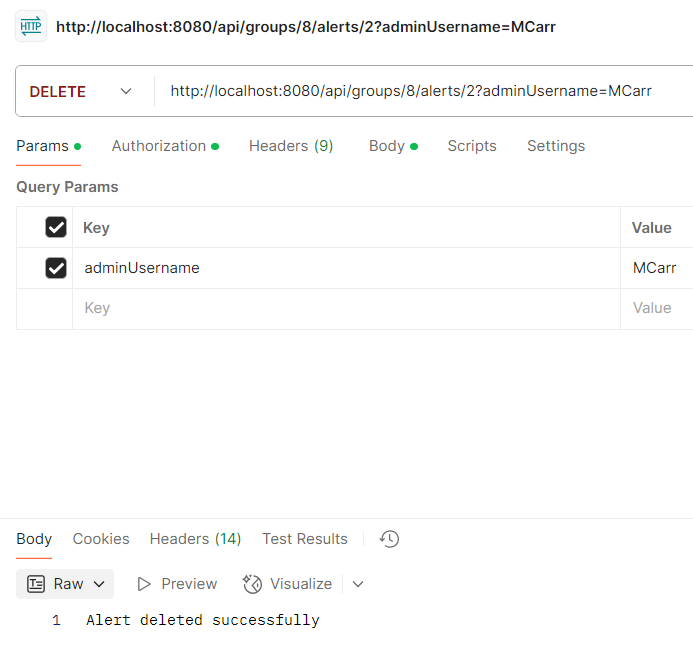
\includegraphics[width=0.9\textwidth]{images/DeleteAlert.png}
    \caption{Risultato API eliminazione Alert}
    \label{fig:api_deleteAlert}
\end{figure}

\paragraph{Visualizza Alert di Gruppo}

\begin{itemize}
    \item \textbf{Endpoint:} \texttt{GET /api/groups/{groupId}/alerts}
    \item \textbf{Descrizione:} Restituisce la lista di tutti gli alerts del gruppo.
\end{itemize}

\begin{figure}[H]
    \centering
    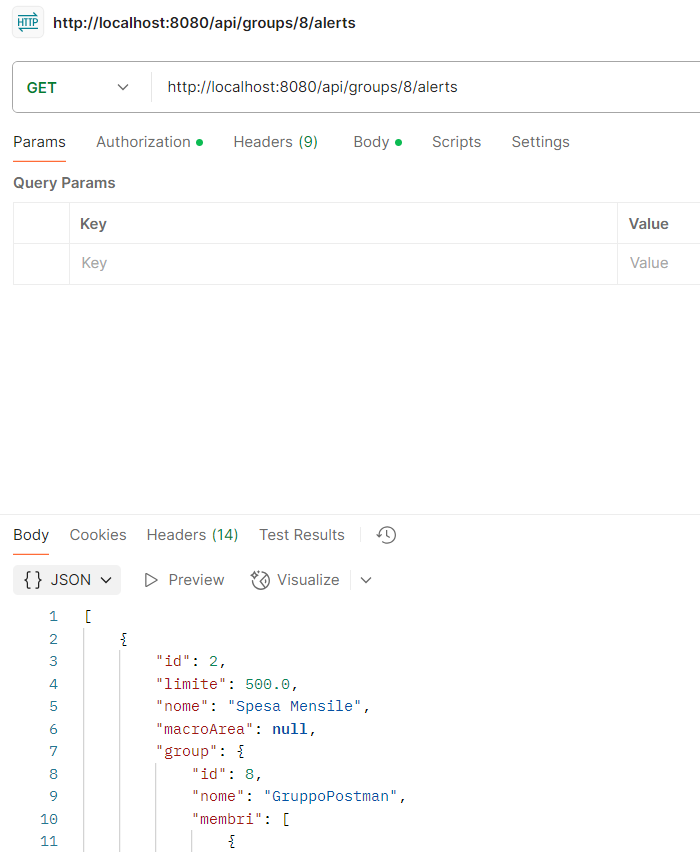
\includegraphics[width=0.9\textwidth]{images/GetAlertsForGroup.png}  
    \caption{Risultato API Visualizzazione Alert di Gruppo}
    \label{fig:api_view_group_alerts}  
\end{figure}
